% =====================================================================
%  LIAR Truth Detector - final report in the CUP Natural Language Engineering (NLE) format.
%  Needs nle.cls / NLE.sty (not included, get it from the course page) in the same folder.
%  Compile with pdfLaTeX (twice). Figures are in ../figures/, tables are in tables.tex
%  (generated by make_tables.py from results/).
% =====================================================================
\documentclass{nle}

\usepackage{graphicx}
\graphicspath{{../figures/}}

\title[Fake news detection on LIAR]
      {Fine-tuned Transformers versus Zero-shot LLMs\\
       for Fake News Detection\\
       \normalsize Evidence from the LIAR benchmark}
\author[Prachi Dhakad and others]
       {\textsc{Prachi Dhakad}, \textsc{Sandhya [Surname]},
        \textsc{Suzzy [Surname]} and \textsc{Arun [Surname]}\\
        [Department], [University], [City], [Country]}

% TODO before submitting: replace the [Surname] and affiliation placeholders above.

\received{Draft, 22 November 2026}
\pagerange{\pageref{firstpage}--\pageref{lastpage}}
\pubyear{2026}

\begin{document}

\label{firstpage}
\maketitle

\begin{abstract}
False claims by public figures spread quickly, and fact-checkers cannot rate every claim by hand. We
build and compare seven models that give a first rating of how true a short political statement is, on
the six-step scale of the LIAR dataset (from \emph{pants-fire} to \emph{true}): a BiLSTM trained from
scratch, BERT and RoBERTa fine-tuned on LIAR (each with and without speaker information), and the
Qwen2.5-7B-Instruct language model used with a prompt but no training (zero-shot and few-shot). Every
model is scored in the same way, on the same 300 test statements, with the same cost model. The best model,
RoBERTa with speaker information, got the exact rating right for 47\hpt 3\% of statements and
separated false-ish from true-ish statements correctly 75\hpt 7\% of the time. From the statement text alone,
BERT and RoBERTa reached 28 to 29\% on six levels. The prompted 7B model was no better than BERT in
accuracy and clearly worse in macro-F1 (0\hpt 183 against 0\hpt 289), while being about 70 times larger and about
45 times more expensive to run. Adding the speaker, party and subject raised accuracy by about 16 points,
but part of that gain comes from a property of the dataset (Section~\ref{sec:leak}). Results rest on one
training run per setting and 300 test statements, so each accuracy is uncertain by about $\pm 5$ points.
\end{abstract}

\section{Introduction}

Many claims in politics are partly true, badly out of context, or simply false. Professional
fact-checkers such as PolitiFact read the evidence and give each claim a rating, but this is slow work. A
tool that gave a quick first guess would help a reviewer decide which claims to look at first. This is
harder than it sounds: a statement such as ``1 percent of Americans are millionaires'' can be true, half
true or misleading depending on facts the model cannot see, so a model has to learn from the wording of a
claim, and sometimes from who said it.

We use the public LIAR benchmark (Wang \shortcite{wang17}), which has about 12,800 statements, each rated by
PolitiFact on six levels. This project asks one main question.
\begin{description}
  \item[RQ.] Is a small model that we fine-tune (about 110 million parameters) better than a big language
        model (7.6 billion parameters) that we only prompt, once we count both accuracy and cost?
\end{description}
To answer it we built a shared data and scoring pipeline, trained a small BiLSTM as a cheap baseline,
fine-tuned BERT and RoBERTa twice each (statement only, and statement plus speaker, party, subject and
credit history), prompted Qwen2.5-7B-Instruct with instructions only and with six examples, and compared
accuracy, macro-F1, time and cost, using a statistical test to check which differences are real.
Our contributions are: a fair and repeatable comparison of seven models with shared labels, seed, test subset,
metrics and cost model; evidence that the fine-tuned model matches or beats the prompted model at a small
fraction of the cost; a measurement of how much speaker information helps, with an explanation of why that
number must be read with care; an analysis of the mistakes, including how the prompted model favours a few
ratings; and a test suite of 99 tests. Code, data and result files are available at
\texttt{https://github.com/arunchowdary-1/Fake-News-Detection-Fine-tuned-Transformers-vs-Zero-shot-LLMs}.

\section{Related work}

\paragraph{The LIAR dataset.} Wang \shortcite{wang17} released LIAR as a larger and more detailed benchmark for
fake news detection than earlier sets. Each statement comes with the speaker, party, subject and a count of
the speaker's past ratings. The paper also tests adding this metadata to a text model, which is the same
question we ask for BERT and RoBERTa.

\paragraph{Recurrent networks and transformers.} LSTMs (\cite{hochreiter97}) read a sentence one word at a
time and keep a memory of what they have seen, and were the standard text model before transformers, so they
make a natural baseline. BERT (Devlin et al.\ \shortcite{devlin19}) is a transformer (\cite{vaswani17}) that
is first trained on a very large amount of text and then fine-tuned for a task with a small amount of labelled
data. RoBERTa (Liu et al.\ \shortcite{liu19}) keeps the same design but is trained for longer on more data.

\paragraph{Prompted language models.} Large language models can do a new task from instructions alone
(zero-shot) or after seeing a few worked examples in the prompt (few-shot) (\cite{brown20}). This avoids
training, but the model is large and slow. We use Qwen2.5-7B-Instruct (Qwen Team \shortcite{qwen24}), run in 4-bit
form (\cite{dettmers23}) so that it fits on a single 16\,GB GPU.

\paragraph{Where our work fits.} We do not propose a new model. We run a careful, like-for-like comparison of
these three families on LIAR and add the cost side, which is often left out.

\section{Data}

LIAR contains short statements that PolitiFact fact-checked, mostly from US politicians and public figures
(speeches, interviews, debates and social media posts). We use the Hugging Face copy of the dataset with its
standard split: 10,269 training, 1,284 validation and 1,283 test statements. Because the 7B model is too slow
to run on all 1,283 test statements, the headline scores use one fixed subset of 300 test statements
(the same rows for every model), chosen so that the mix of ratings matches the full test set (22 pants-fire,
59 false, 50 barely-true, 62 half-true, 58 mostly-true and 49 true). Full-test numbers are reported where we
have them.

Every statement has one of six ratings, from least to most truthful: \emph{pants-fire}, \emph{false},
\emph{barely-true}, \emph{half-true}, \emph{mostly-true} and \emph{true}. Figure~\ref{fig:dist} shows that the
ratings are fairly balanced except for \emph{pants-fire}, which is much rarer. Each statement also comes with
the speaker, job title, state, party (for example republican 4,510 training rows, democrat 3,345), subject (for
example economy 896), the context, and five \emph{credit-history} counts of the speaker's past statements
rated barely-true, false, half-true, mostly-true and pants-on-fire. The training set has 2,916 different
speakers, and many speakers appear many times, which is one reason that knowing the speaker helps a model.

\begin{figure}
\centering
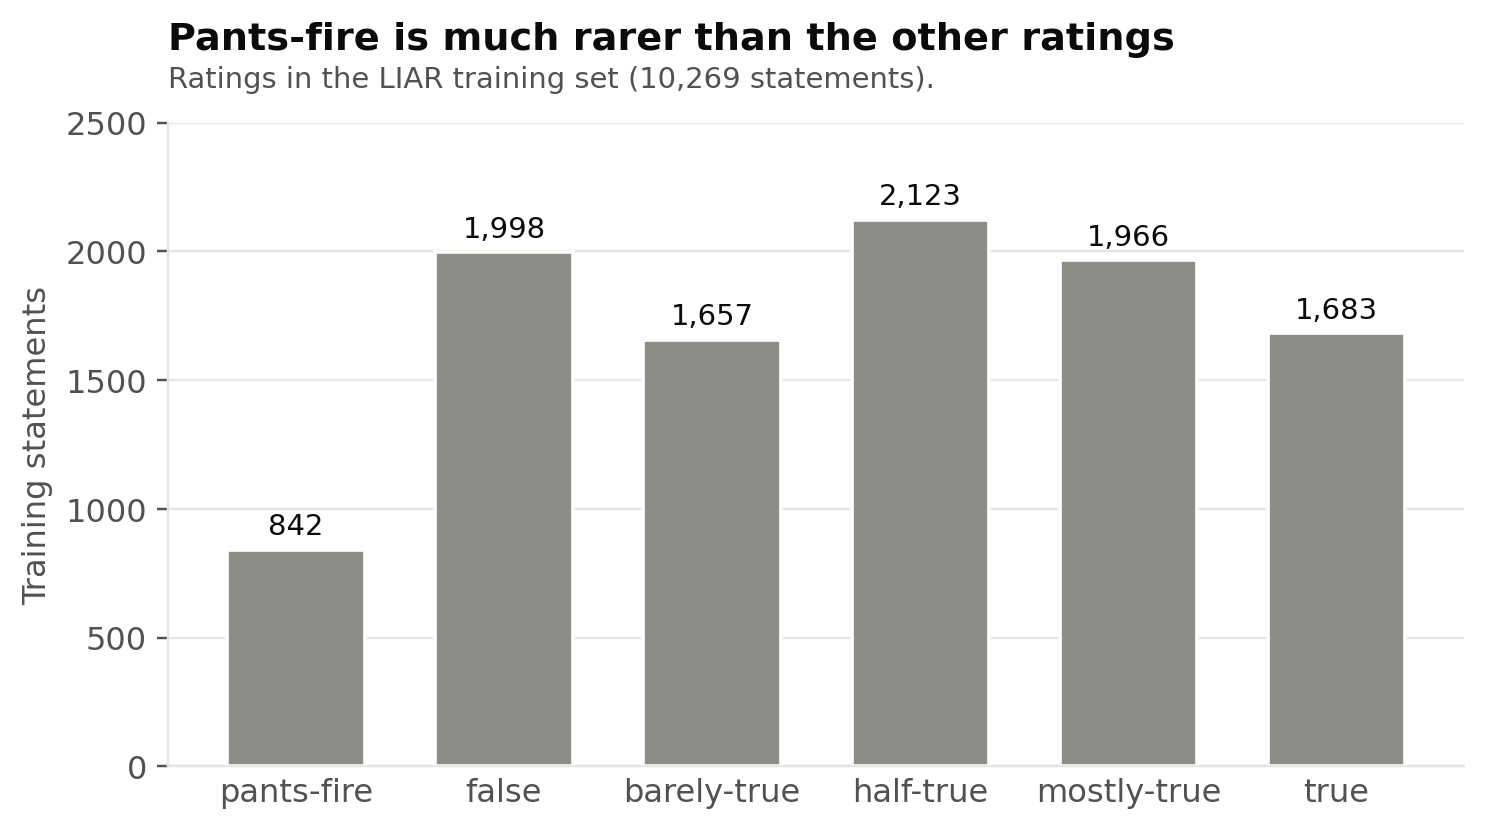
\includegraphics[width=0.85\textwidth]{fig_label_distribution.png}
\caption{Number of training statements per rating.}
\label{fig:dist}
\end{figure}

\paragraph{A property of the data that matters later.} In the LIAR release, the five credit-history counts
include the rating of the current statement itself, so a model can see part of the answer in the speaker's
history. We return to this in Section~\ref{sec:leak}. All statements are short, English and political, and nearly
all are from the United States, so we make no claim about other kinds of news.

\section{Experimental setup}

\subsection{Keeping the comparison fair}
We fixed the following for all models: the same six labels in the same order; random seed 42; the same 300-statement
test subset; one shared function for accuracy, macro-F1 and the confusion matrix; and one cost model, in which
every model is priced as if it ran on a Tesla T4 GPU at \$0\hpt 35 per hour plus 10\% overhead, one statement at a
time (batch size 1). Random guessing scores 16\hpt 7\% on six levels, and always answering the most common
rating in the subset (half-true) scores 20\hpt 7\%. For the fake-vs-real view, always guessing the more common
side scores 56\hpt 3\%. With only 300 statements, each accuracy is uncertain by about $\pm 5$ points.

\subsection{Models}
Table~\ref{tab:models} lists the models and the pre-trained checkpoints they start from. All checkpoints are
published on the Hugging Face Hub.

\begin{table}
\caption{Models, pre-trained checkpoints and how each was used.}
\begin{minipage}{\textwidth}
\begin{tabular}{llll}
\hline\hline
Model & Hugging Face ID & Source & Use \\
\hline
BiLSTM & none & built by us & trained from scratch \\
BERT & \texttt{bert-base-uncased} & Google & fine-tuned on LIAR \\
RoBERTa & \texttt{roberta-base} & Meta & fine-tuned on LIAR \\
Qwen2.5-7B & \texttt{Qwen/Qwen2.5-7B-Instruct} & Qwen team, Alibaba & prompted only, 4-bit FP4 \\
\hline\hline
\end{tabular}
\vspace{-1.5\baselineskip}
\end{minipage}
\label{tab:models}
\end{table}

\paragraph{BiLSTM baseline.} The BiLSTM starts with no knowledge of language. It reads the statement in both
directions, combines the final state with the strongest signal from any word, and outputs six scores. It uses
word vectors of size 100 learned from scratch (vocabulary of at most 20,000 words seen at least twice in the
training set only, so nothing leaks from the test set), one bidirectional LSTM layer with 128 units per
direction, dropout 0.5, statements cut at 64 words, the Adam optimiser with learning rate $10^{-3}$, batch size 64,
up to 15 epochs with early stopping after 3 epochs without improvement (best epoch 6), and class weights in the
loss. It has 932,998 trainable parameters and trains on a CPU in about 4 minutes.

\paragraph{BERT and RoBERTa.} We fine-tuned \texttt{bert-base-uncased} (109\hpt 5M parameters) and
\texttt{roberta-base} (124\hpt 7M parameters) with a new six-way output layer, each twice. In the
\emph{text-only} runs the input is the statement (up to 128 tokens). In the \emph{speaker-information} runs the speaker,
party, subject and credit history are written in front of the statement (up to 256 tokens), for example
``\texttt{speaker: dwayne-bohac | party: republican | subject: abortion | history: 0,1,0,0,0 [SEP] Says the
Annies List political group supports third-trimester abortions on demand.}'' The setup was identical for all four
runs: AdamW (Loshchilov and Hutter \shortcite{loshchilov19}) with learning rate $2\times 10^{-5}$ and weight
decay 0\hpt 01, batch size 16, 3 epochs, 10\% warm-up followed by a linear decrease, gradient clipping at 1\hpt 0,
fp16 arithmetic, and inverse-frequency class weights. The best epoch was chosen by macro-F1 on the validation
set, and was the last epoch in every run. We used the Transformers library (Wolf et al.\ \shortcite{wolf20}) on a
Colab Tesla T4.

\paragraph{Prompted Qwen2.5-7B-Instruct.} We used the model without any training, in 4-bit form (FP4 from the
bitsandbytes library) on a Kaggle Tesla T4. The \emph{zero-shot} prompt is a system message that tells the model
it is a fact-checking expert, lists the six labels and says ``Respond with ONLY the label, nothing else'' (full
text in Appendix~\ref{app:prompt}); the statement follows. The \emph{few-shot} prompt adds six worked examples
(one per rating) taken from the training set with seed 42, each 60 to 200 characters long and shuffled so that the
last example does not favour one rating; because they come from the training set, none can appear in the test
subset. Decoding is greedy with at most 12 new tokens, so runs are repeatable. Parsing is strict: an answer counts
only if it contains exactly one valid label (``pants on fire'' is accepted as pants-fire, but a negation such as
``not true'' or two labels are rejected). A rejected answer is marked \emph{invalid} and counted as wrong, so
parsing never raises the score. Each prompt was written once and run once; a 20-statement test checked only that the
output could be parsed. The model saw the statement only, not the speaker or party.

\subsection{Metrics and statistical test}
\emph{Accuracy} is the share of statements given exactly the right rating. \emph{Macro-F1} averages the F1 score of
each of the six ratings, so a model cannot score well by favouring a few common ratings. For the
\emph{fake-vs-real view} we group pants-fire, false and barely-true as false-ish and the other three as true-ish;
this grouping is our own choice and was not part of training. To tell real differences from luck we use McNemar's
exact test (\cite{mcnemar47}), which looks only at the statements where two models disagree and asks whether one wins
more often than chance would allow.

\section{Results}

\subsection{Overall accuracy}
Table~\ref{tab:main} gives every score on the shared 300-statement subset, and Figures~\ref{fig:acc6} and
\ref{fig:acc2} show the exact-rating accuracy and the fake-vs-real view. RoBERTa with speaker information is best
(0\hpt 473 accuracy, 75\hpt 7\% fake vs real), followed by BERT with speaker information. With the statement alone,
BERT and RoBERTa reach 0\hpt 293 and 0\hpt 283 (28 to 29\%), above the prompted 7B model, the BiLSTM and chance.

% Generated by report/nle/make_tables.py from results/. Do not edit by hand.

\begin{table}
\caption{Main results on the shared 300-statement test subset. The fake-vs-real column is our own grouping of the saved predictions. The BiLSTM was timed on a CPU.}
\begin{minipage}{\textwidth}
\begin{tabular}{lcccc}
\hline\hline
Model & Accuracy & Macro-F1 & Fake vs real & Invalid answers \\
\hline
RoBERTa + speaker info & 0\hpt 473 & 0\hpt 483 & 75\hpt 7\% & 0 / 300 \\
BERT + speaker info & 0\hpt 457 & 0\hpt 470 & 75\hpt 3\% & 0 / 300 \\
BERT, text only & 0\hpt 293 & 0\hpt 289 & 64\hpt 0\% & 0 / 300 \\
RoBERTa, text only & 0\hpt 283 & 0\hpt 282 & 63\hpt 0\% & 0 / 300 \\
Qwen 7B few-shot & 0\hpt 250 & 0\hpt 183 & 59\hpt 0\% & 0 / 300 \\
BiLSTM & 0\hpt 190 & 0\hpt 173 & 56\hpt 3\% & 0 / 300 \\
Qwen 7B zero-shot & 0\hpt 167 & 0\hpt 126 & 56\hpt 7\% & 1 / 300 \\
\hline\hline
\end{tabular}
\par\smallskip{\small Random guessing: 16\hpt 7\% (six levels). Always guessing one side: 56\hpt 3\% (fake vs real).}
\vspace{-1.5\baselineskip}
\end{minipage}
\label{tab:main}
\end{table}

\begin{table}
\caption{Results on the full test set (1,283 statements).}
\begin{minipage}{\textwidth}
\begin{tabular}{lcc}
\hline\hline
Model & Accuracy & Macro-F1 \\
\hline
RoBERTa + speaker info & 0\hpt 461 & 0\hpt 467 \\
BERT + speaker info & 0\hpt 449 & 0\hpt 457 \\
RoBERTa, text only & 0\hpt 288 & 0\hpt 291 \\
BERT, text only & 0\hpt 273 & 0\hpt 277 \\
BiLSTM & 0\hpt 212 & 0\hpt 201 \\
\hline\hline
\end{tabular}
\vspace{-1.5\baselineskip}
\end{minipage}
\label{tab:full}
\end{table}

\begin{table}
\caption{McNemar exact tests on the 300 statements. ``Only A right'' counts the statements that A got right and B got wrong.}
\begin{minipage}{\textwidth}
\begin{tabular}{llccc}
\hline\hline
Model A & Model B & Only A right & Only B right & $p$-value \\
\hline
Qwen few-shot & Qwen zero-shot & 48 & 23 & 0\hpt 004 \\
BERT text only & Qwen few-shot & 66 & 53 & 0\hpt 27 \\
BERT text only & Qwen zero-shot & 75 & 37 & 0\hpt 0004 \\
BERT + speaker info & BERT text only & 83 & 34 & $<$0\hpt 0001 \\
RoBERTa text only & BERT text only & 30 & 33 & 0\hpt 80 \\
RoBERTa + speaker info & BERT + speaker info & 30 & 25 & 0\hpt 59 \\
\hline\hline
\end{tabular}
\vspace{-1.5\baselineskip}
\end{minipage}
\label{tab:sig}
\end{table}

\begin{table}
\caption{Size, time and cost, priced at a T4 GPU rate of \$0.35 per hour plus 10\% overhead, batch size 1.}
\begin{minipage}{\textwidth}
\begin{tabular}{lrrrrr}
\hline\hline
Model & Params & Train (min) & Sec per 1,000 & \$ per 1,000 & GPU (MB) \\
\hline
BiLSTM (CPU) & 1M & 3\hpt 9 & 2\hpt 1 & 0\hpt 0002 & n/a \\
BERT, text only & 109M & 3\hpt 2 & 14\hpt 7 & 0\hpt 0016 & 2,144 \\
BERT + speaker info & 109M & 3\hpt 8 & 13\hpt 9 & 0\hpt 0015 & 2,301 \\
RoBERTa, text only & 125M & 3\hpt 4 & 14\hpt 4 & 0\hpt 0015 & 2,429 \\
RoBERTa + speaker info & 125M & 3\hpt 9 & 17\hpt 3 & 0\hpt 0018 & 2,502 \\
Qwen 7B zero-shot & 7,616M & none & 393\hpt 5 & 0\hpt 0421 & 5,743 \\
Qwen 7B few-shot & 7,616M & none & 661\hpt 3 & 0\hpt 0707 & 5,789 \\
\hline\hline
\end{tabular}
\vspace{-1.5\baselineskip}
\end{minipage}
\label{tab:cost}
\end{table}


\begin{figure}
\centering
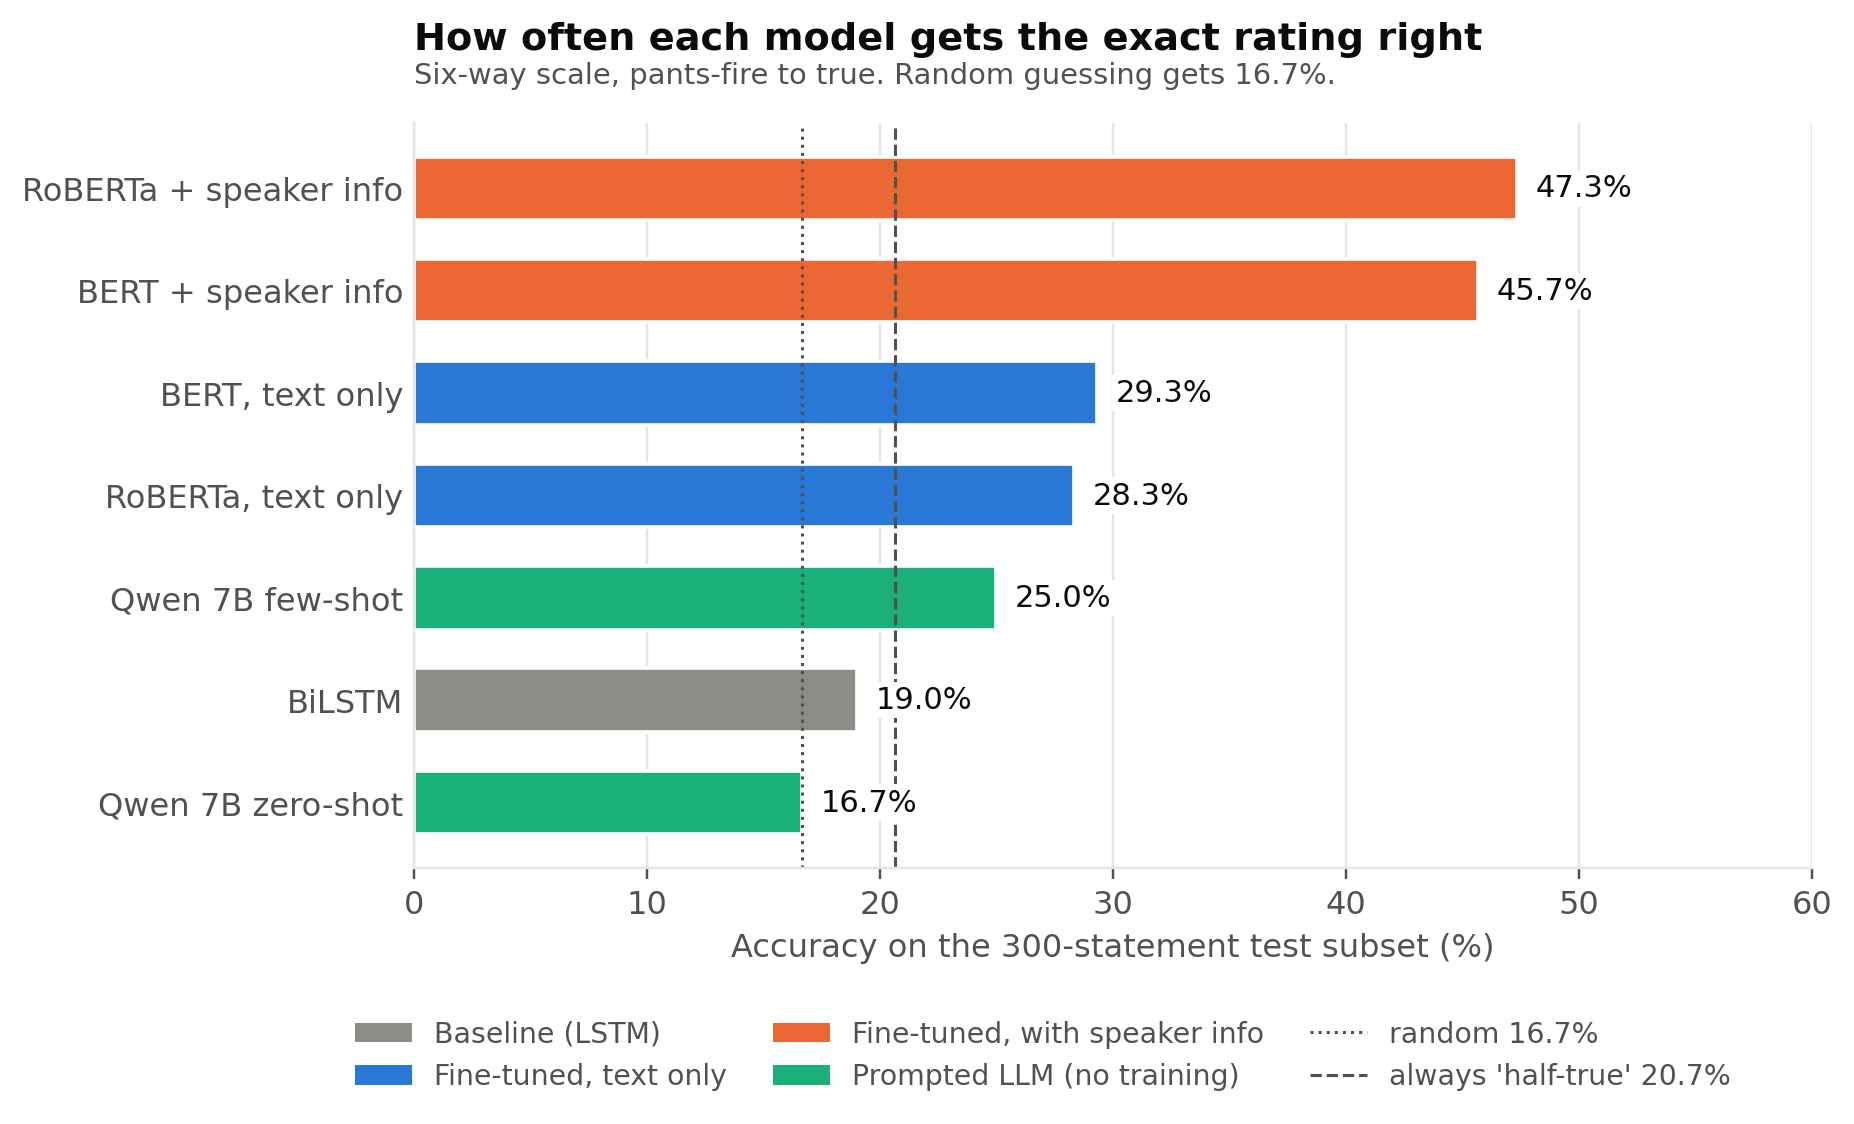
\includegraphics[width=\textwidth]{fig_accuracy_6way.png}
\caption{Exact-rating accuracy on the six-level scale. Colours show the kind of model.}
\label{fig:acc6}
\end{figure}

\begin{figure}
\centering
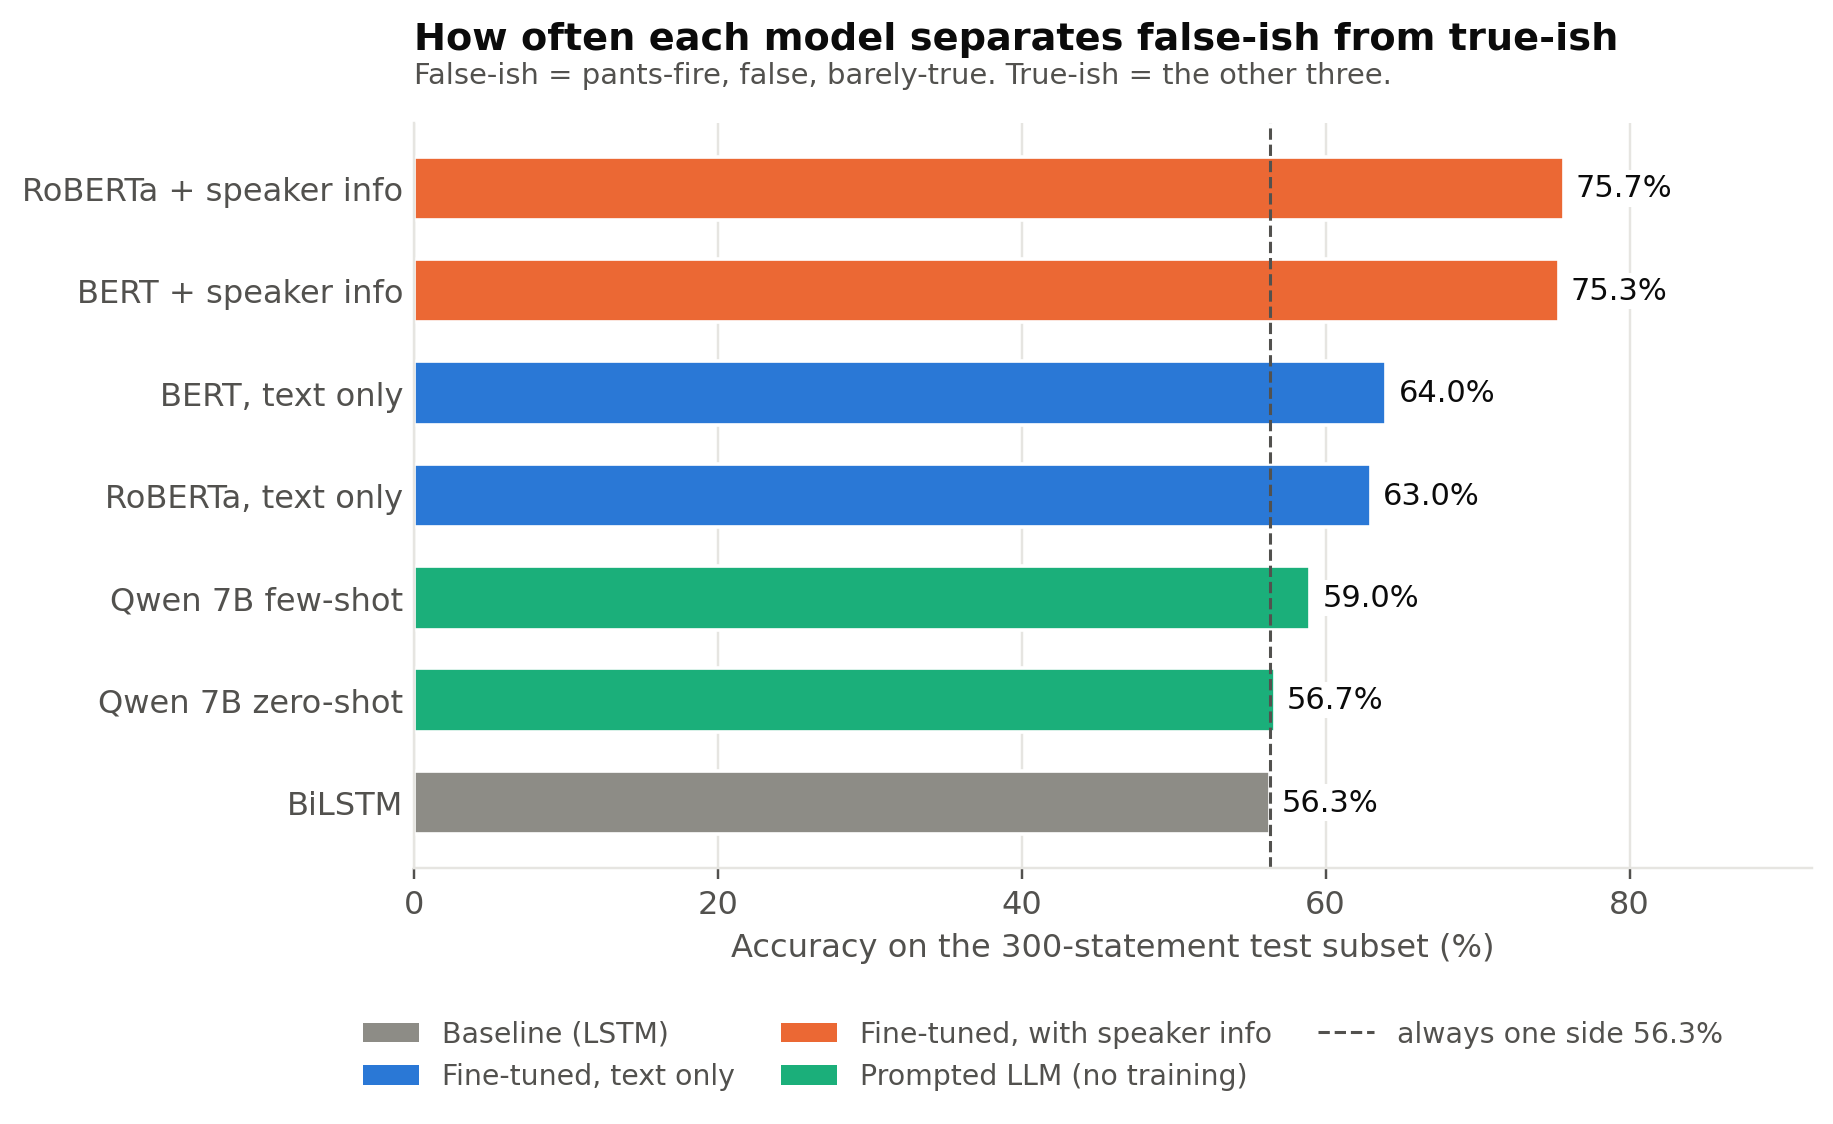
\includegraphics[width=\textwidth]{fig_accuracy_2way.png}
\caption{Accuracy when the six ratings are grouped into false-ish and true-ish.}
\label{fig:acc2}
\end{figure}

\subsection{Full test set}
The 300-statement subset is small, so we also scored the fine-tuned models and the BiLSTM on all 1,283 test
statements (Table~\ref{tab:full}). The numbers agree closely with the subset, which gives us more confidence in
them. The prompted model could not be run on the full set because it is too slow.

\subsection{Which ratings are found, and which are missed}
Figure~\ref{fig:recall} shows, for RoBERTa, how many statements of each real rating the model got right. Speaker
information raises the score for five of the six ratings. The exception is \emph{true}, where it falls from 47\% to
29\%. Without speaker information the model finds only 10\% of the half-true statements, the hardest rating for
every model. Figure~\ref{fig:conf} shows where the mistakes go: most wrong answers land on a neighbouring level, for
example \emph{mostly-true} called \emph{true}, and between 42\% and 54\% of all errors are of this near-miss kind.
Two statements rated half-true that the text-only RoBERTa called true show how hard the middle ratings are: a
Facebook post that ``1 percent of Americans are millionaires. 47 percent of House Reps.\ are millionaires.
56 percent of Senators are millionaires'', and Nikki Haley's claim that ``President Obama and his National Labor
Relations Board sued Boeing over its decision to open a plant in South Carolina''. Both are true in part and
misleading in part, so even a careful human would need the evidence to decide.

\begin{figure}
\centering
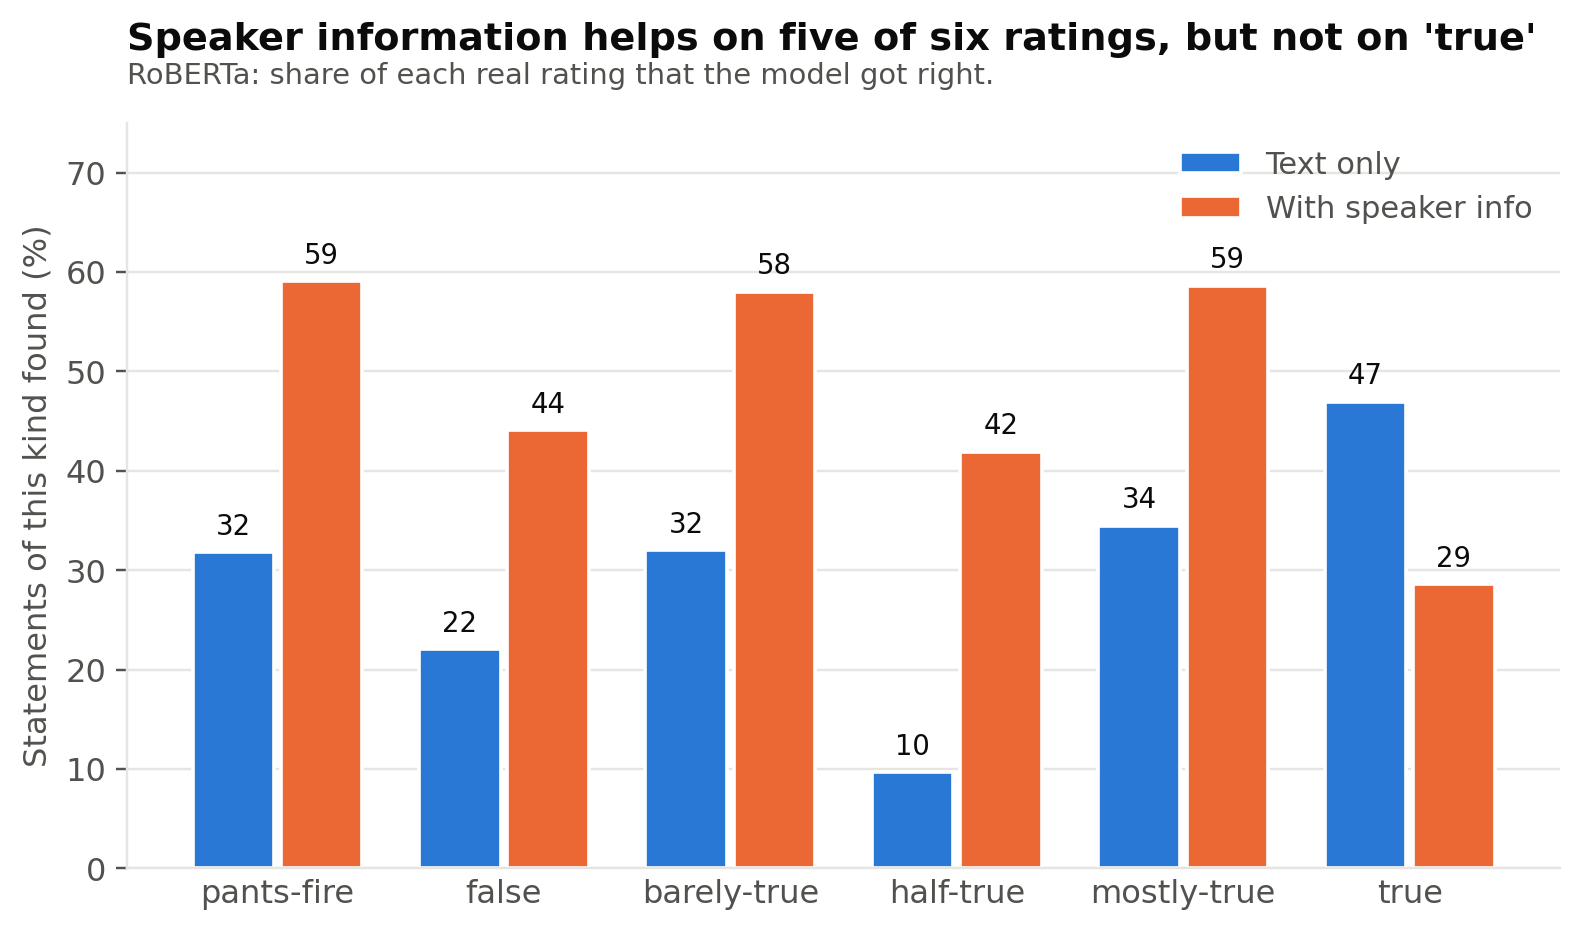
\includegraphics[width=0.9\textwidth]{fig_recall_by_class.png}
\caption{Share of each real rating found by RoBERTa, with and without speaker information (300 statements).}
\label{fig:recall}
\end{figure}

\begin{figure}
\centering
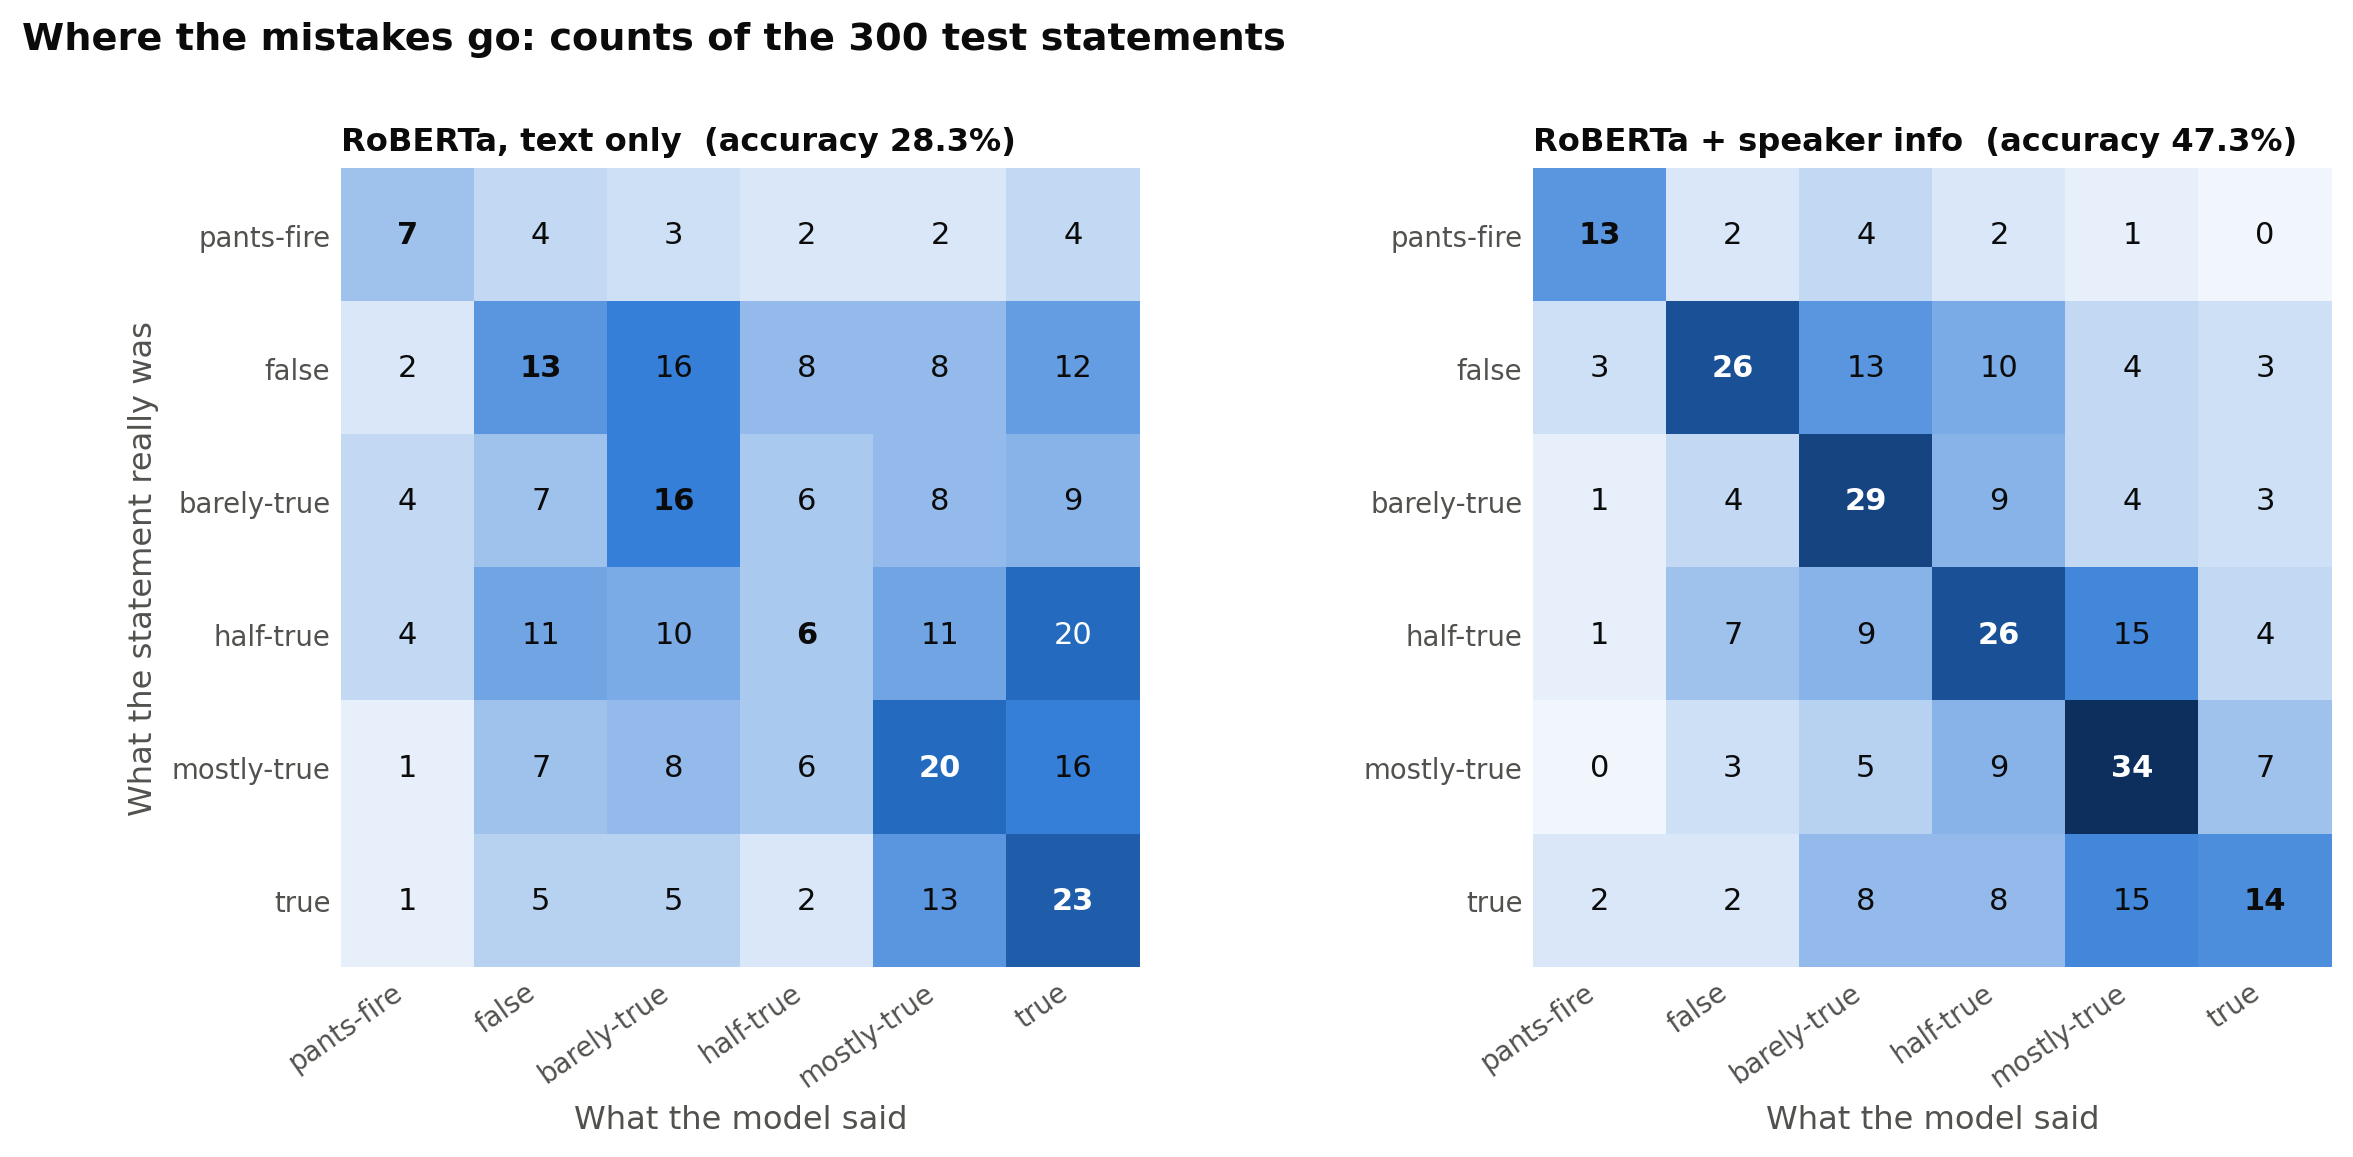
\includegraphics[width=\textwidth]{fig_confusion.png}
\caption{Confusion matrices for RoBERTa. Rows are the real rating, columns are the model's answer.}
\label{fig:conf}
\end{figure}

\subsection{How the prompted model goes wrong}
The prompted model does not spread its answers over the six ratings (Figure~\ref{fig:bias}). Zero-shot, it answered
\emph{pants-fire} for 136 of the 300 statements (45\%), although only 22 really are pants-fire, and it almost never
said \emph{true} or \emph{barely-true}. Few-shot moved the bias: it answered \emph{false} for 146 statements (49\%)
and never answered \emph{mostly-true}. Six examples helped, but they did not remove the bias.

\begin{figure}
\centering
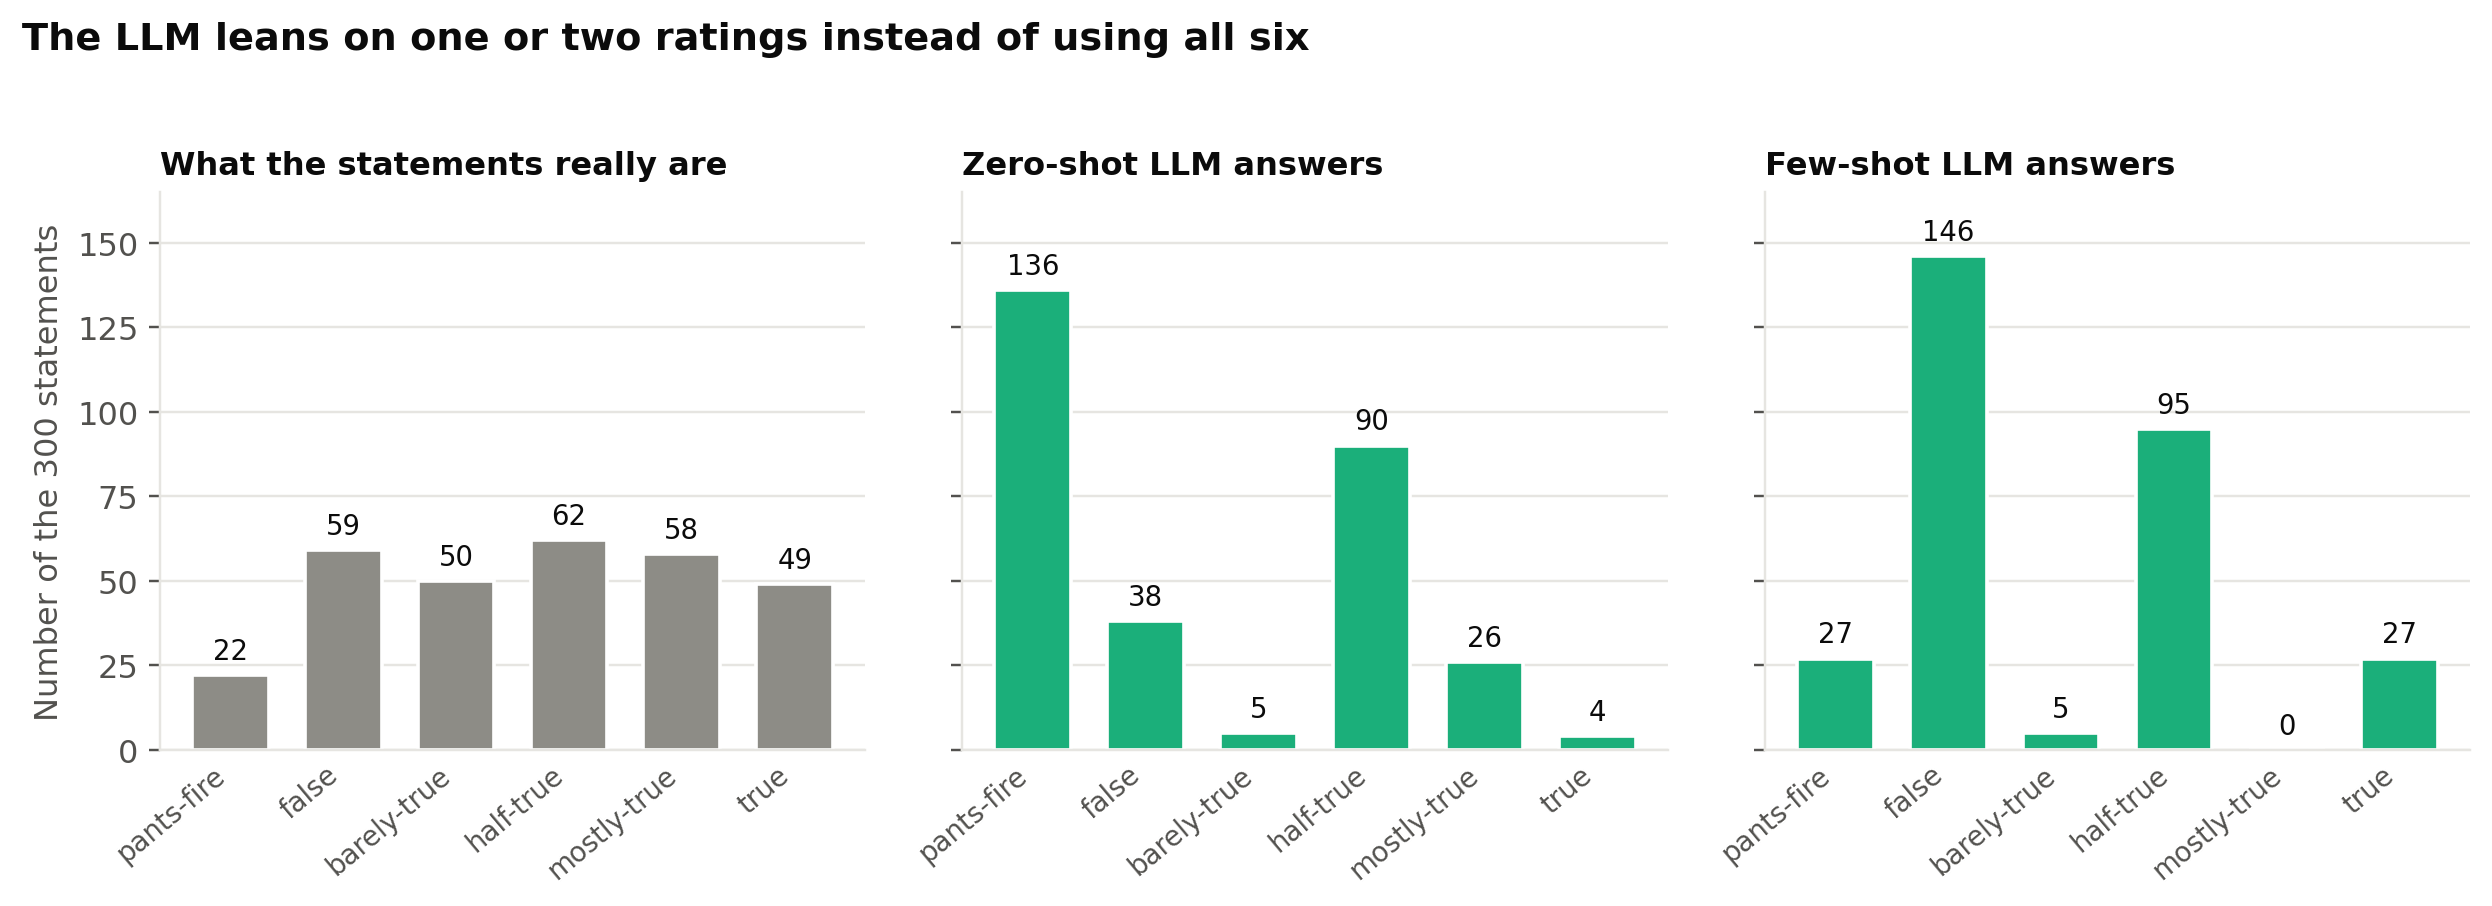
\includegraphics[width=\textwidth]{fig_llm_bias.png}
\caption{What the 300 statements really are (left) and what the prompted model answered, zero-shot (middle) and
few-shot (right).}
\label{fig:bias}
\end{figure}

\subsection{Are the differences real?}
Table~\ref{tab:sig} gives McNemar tests. Few-shot beats zero-shot ($p=0\hpt 004$), so the six examples helped and
this is unlikely to be luck. Zero-shot is clearly worse than BERT ($p=0\hpt 0004$) and sits at chance level. BERT
against few-shot is not significant in accuracy ($p=0\hpt 27$): the 4-point gap is within the noise of 300 statements,
and the difference shows up in macro-F1 (0\hpt 289 against 0\hpt 183) because the prompted model favours a few
ratings. Speaker information gives a big, real gain ($p<0\hpt 0001$). BERT and RoBERTa are tied: their differences
are about one point and well inside the noise, so we do not claim one is better.

\subsection{Cost and speed}
Table~\ref{tab:cost} and Figure~\ref{fig:cost} compare size, training time, speed and cost. Compared with the better
prompted run (few-shot), text-only BERT is about 70 times smaller, about 45 times faster and about 45 times cheaper
per prediction, and it scores 0\hpt 106 higher in macro-F1. BERT's one-off training cost of about \$0\hpt 02 is paid
back after roughly 300 predictions. These ratios are an upper bound: we ran the prompted model one statement at a
time, and a batching server such as vLLM would narrow the gap.

\begin{figure}
\centering
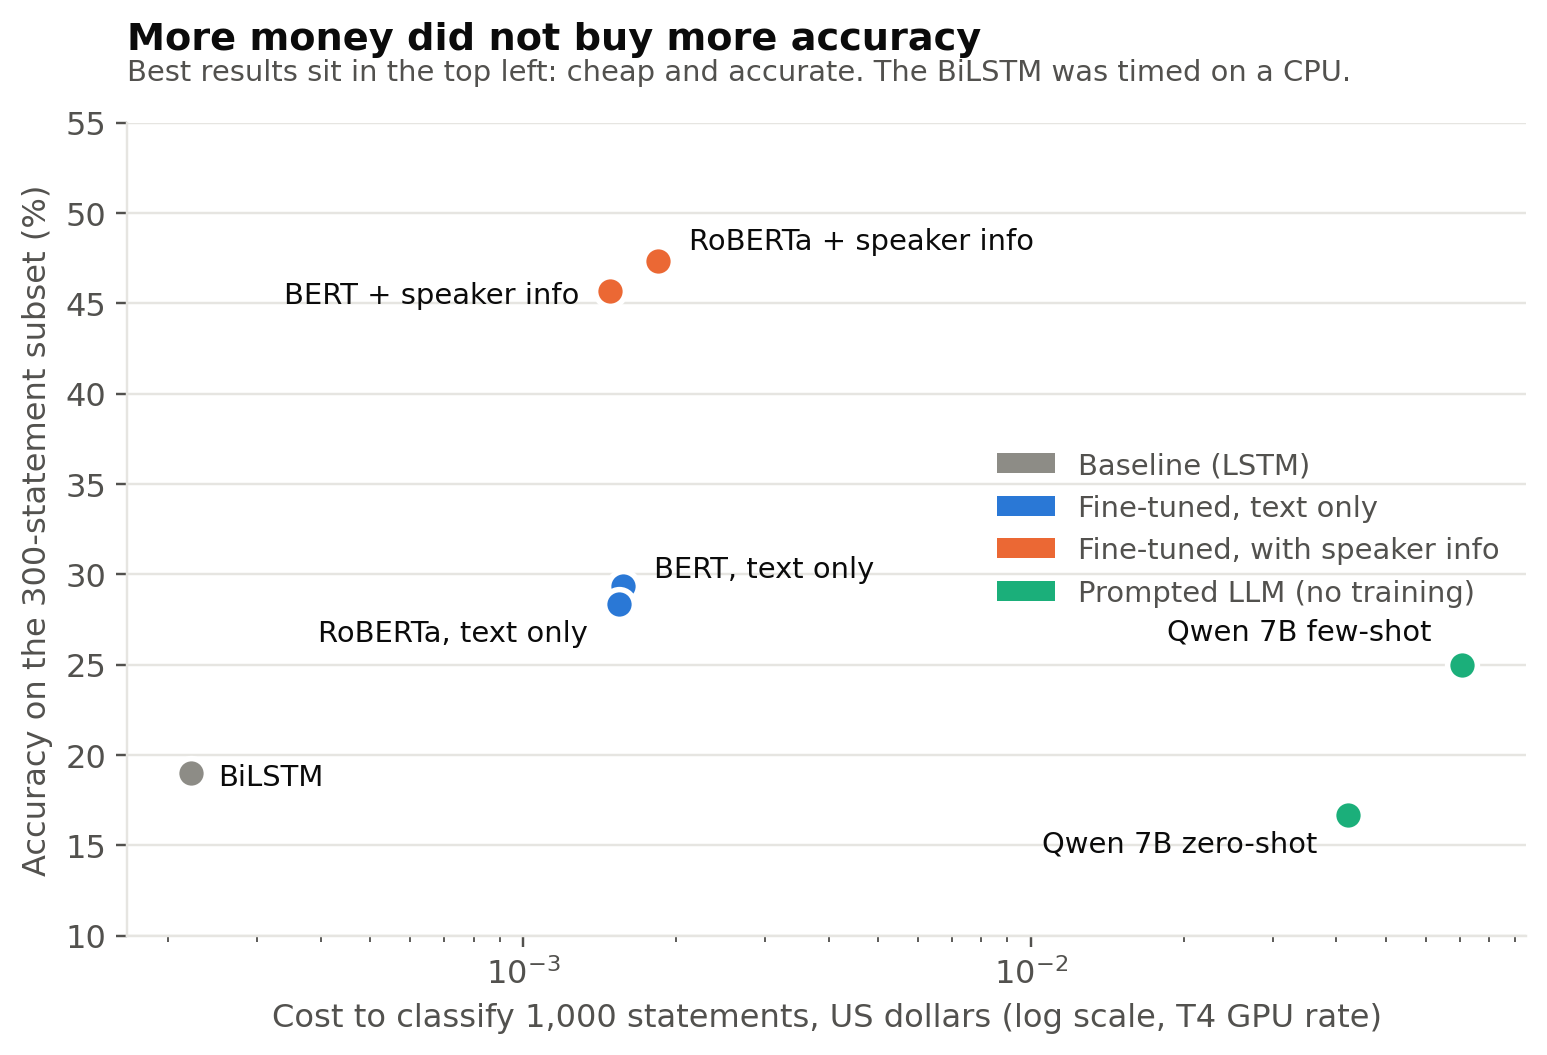
\includegraphics[width=0.95\textwidth]{fig_cost_accuracy.png}
\caption{Cost against accuracy. The best models are in the top left: cheap and accurate. The BiLSTM was timed on a CPU.}
\label{fig:cost}
\end{figure}

\section{Discussion}\label{sec:disc}

\subsection{What worked} Pre-training matters: the BiLSTM, which starts from nothing, scored 19\% and is barely above
guessing the common class, while BERT and RoBERTa scored 28 to 29\% from the same statements. Fine-tuning beat
prompting here: a few minutes of training on 10,000 labelled statements taught the small model the six-level scale
better than instructions and six examples taught the large one. Knowing the speaker helped a lot, the largest single
effect we measured, for only about 30 seconds more training time. BERT and RoBERTa behave the same, so the choice
between them does not matter much for this task.

\subsection{Why the prompted model struggled} The six levels are subtle: the gap between barely-true, half-true and
mostly-true depends on small details and on evidence the model does not have. An instruction-following model with no
task data seems to turn ``sounds dubious'' into \emph{false} or \emph{pants-fire}, and has no sense of where the
middle ratings begin. A fine-tuned model learns those boundaries from thousands of examples. We tried one model, one
prompt and 4-bit weights, so a different setup might do better, but we did not test it.

\subsection{An important caveat about the best result}\label{sec:leak}
\textbf{Read this before quoting the 47\% or the 75\%.} The five credit-history numbers are the speaker's record of
past ratings, and in the LIAR release they already include the rating of the current statement, so a model can
partly read the answer from the speaker's history. The best result is best described as the value of knowing who is
speaking, not as a better understanding of the claim. That is why the fair comparison with the prompted model, which
sees only the statement, is the text-only models. On a brand-new statement, where no such history exists, we should
expect results closer to the text-only numbers. The cleaner test, using speaker, party and subject without the history
counts, has not been run and is the first thing we would add.

\subsection{What this means for detecting fake news} As a first-pass signal the models are useful: on fake vs real
the best model is right about three times out of four against a baseline of 56\%, and the text-only models reach about
64\%. As an automatic judge they are not good enough: the best text-only model gets the exact rating right fewer than
three times in ten, so a person should read anything that matters. Many errors move a claim by one level, which is much
less harmful than calling a false claim true. If the speaker is known we would use RoBERTa or BERT with speaker
information (checking the caveat above before quoting its accuracy), and if only the text is known text-only BERT,
which matches or beats the prompted 7B model at about one forty-fifth of the cost. We do not recommend the prompted
7B model for this task as we set it up: it is slower, costlier and no better.

\subsection{Bugs found and fixed}\label{sec:bugs} Running the code on the real dataset, and reviewing each other's pull requests,
caught problems that reading the code did not. The Hugging Face copy of LIAR numbers its labels in a different order
from ours (labels are now mapped by name, otherwise every confusion matrix would have been scrambled); the metadata
text looked for a field that does not exist, so every row said ``history: 0,0,0,0,0''; the test subset had 50
statements per rating and is now proportional (the BiLSTM was re-run on it); and the LLM runs used 4-bit FP4 and not
NF4 as first documented.

\section{Limitations and ethics}

\paragraph{Limitations.} The data is short, English, US political statements, and we expect worse results on other
topics, countries, languages and full articles. Three hundred statements means about $\pm 5$ points on any accuracy,
and the prompted model was scored only on this subset. We used a single random seed and one run per setting, so
run-to-run variation is not measured. The history counts include the answer (Section~\ref{sec:leak}). We tested one
prompted model with one prompt and 4-bit weights; other models (for example Mistral-7B), other prompts, retrieved
examples or fine-tuning the model (QLoRA) could close some of the gap, and it never saw the speaker, so it did not get
the same information as the speaker-aware models. The last epoch was the best for BERT and RoBERTa, so a longer run may
add a little. Absolute accuracy is modest, which is normal for LIAR, where text-only models usually score about 25 to
30\% on six levels. The planned demo application (a FastAPI service and a simple front end) is not in the repository.

\paragraph{Ethical considerations.} The labels are human opinions: PolitiFact ratings involve judgement, and the model
learns those judgements, including any bias in them. A model that uses who spoke can learn that some people or parties
are ``usually false''; that may be statistically true in the data and still unfair to a particular claim, so the
speaker-aware models should not be used to rate individual people's statements automatically. Mistakes can damage a
reputation or spread a wrong belief, so we recommend using the model only to help a human reviewer prioritise, with a
human making the final call. Our best six-level accuracy is under 50\%, and the fake-vs-real figure should be quoted
only with its grouping and the history caveat. LIAR is a public dataset; we used no private or personal data and no
secrets are stored in the code.

\section{Conclusion and future work}

We built and compared seven models for rating the truthfulness of political statements. A small, fine-tuned model was
as accurate as a prompted 7B model and clearly better in macro-F1, while being about 70 times smaller and 45 times
cheaper. Adding the speaker raised accuracy from about 29\% to about 46\%, giving a best result of 47\hpt 3\% on six
levels and 75\hpt 7\% on fake vs real, but this partly reflects the credit-history counts. Statement text alone gives 28 to
29\% on six levels, which is typical for this hard dataset. The main lesson is that, for a narrow task with labelled
data, training a small model is better than prompting a large one, both in quality and in cost, and the model is a
helper for human reviewers, not a replacement for them. Future work: run the test with speaker, party and subject but
without the history counts; build the demo application; train on more varied data to widen the scope beyond US
politics; repeat each run with several seeds and score the prompted model on more statements; try other models and
prompts, retrieved examples and QLoRA; and measure speaker bias directly, for example by comparing results across
parties.

\appendix

\section{Training settings}\label{app:settings}

\begin{table}
\caption{Settings for every trained model.}
\begin{minipage}{\textwidth}
\begin{tabular}{lccc}
\hline\hline
Setting & BiLSTM & BERT / RoBERTa & Qwen 7B \\
\hline
Training data & train split & train split & none \\
Optimiser & Adam & AdamW & not trained \\
Learning rate & 0\hpt 001 & $2\times 10^{-5}$ & -- \\
Batch size & 64 & 16 & 1 (inference) \\
Epochs (max) & 15 & 3 & -- \\
Early stopping & 3 epochs & 2 epochs & -- \\
Best epoch & 6 & 3 & -- \\
Max length & 64 words & 128 / 256 tokens & 12 new tokens \\
Class weights & yes & yes & -- \\
Seed & 42 & 42 & 42 (few-shot picks) \\
Hardware & CPU & Colab T4 & Kaggle T4 \\
Precision & fp32 & fp16 & 4-bit FP4 \\
\hline\hline
\end{tabular}
\vspace{-1.5\baselineskip}
\end{minipage}
\end{table}

\section{The prompt}\label{app:prompt}
The system message used for both prompted runs was: \emph{You are a fact-checking expert. Classify the given political
statement by its truthfulness using exactly one of these labels: pants-fire (ridiculously false), false, barely-true,
half-true, mostly-true, true. Respond with ONLY the label, nothing else.} Each statement is then given as
``Statement: \ldots{} Label:''. The few-shot run places six worked examples as earlier question-and-answer turns in the
same format.

\section{How the work was organised}
We tracked the work as GitHub issues (data, evaluation, each model, analysis and documentation), each done on its own
branch and merged through a pull request. Teammates reviewed each other's pull requests, and several of the bugs
listed in Section~\ref{sec:bugs} were found that way. The shared pieces (labels, data loader, scoring code, test subset) were built
first so the model work could run in parallel.

\section{How to reproduce the results}
Install the packages in \texttt{requirements.txt}, then run \texttt{python -m pytest tests/ -q} (all 99 tests pass) and
\texttt{python -m baselines.train} for the BiLSTM (a CPU is enough). BERT, RoBERTa and the prompted runs need a GPU (a
Colab or Kaggle T4 is enough); the notebooks are in \texttt{notebooks/}. Results are written to \texttt{results/}, the
cost table is \texttt{results/cost\_comparison.md}, the tables of this report are rebuilt with
\texttt{python report/nle/make\_tables.py}, and the figures with \texttt{python report/make\_figures.py}.

\label{lastpage}

\begin{thebibliography}{}
\bibitem[\protect\citename{Brown {\it et al.}\ }2020]{brown20}
 Brown, T. {\it et al.}\ (2020) Language models are few-shot learners. {\it Advances in Neural Information
 Processing Systems\/} {\bf 33}. arXiv:2005.14165.
\bibitem[\protect\citename{Dettmers {\it et al.}\ }2023]{dettmers23}
 Dettmers, T., Pagnoni, A., Holtzman, A. and Zettlemoyer, L. (2023) QLoRA: efficient finetuning of quantized LLMs.
 {\it Advances in Neural Information Processing Systems\/} {\bf 36}. arXiv:2305.14314.
\bibitem[\protect\citename{Devlin {\it et al.}\ }2019]{devlin19}
 Devlin, J., Chang, M.-W., Lee, K. and Toutanova, K. (2019) BERT: pre-training of deep bidirectional transformers
 for language understanding. In {\it Proceedings of NAACL}, pp.~4171--4186. arXiv:1810.04805.
\bibitem[\protect\citename{Hochreiter and Schmidhuber }1997]{hochreiter97}
 Hochreiter, S. and Schmidhuber, J. (1997) Long short-term memory. {\it Neural Computation\/} {\bf 9}(8): 1735--1780.
\bibitem[\protect\citename{Liu {\it et al.}\ }2019]{liu19}
 Liu, Y. {\it et al.}\ (2019) RoBERTa: a robustly optimized BERT pretraining approach. arXiv:1907.11692.
\bibitem[\protect\citename{Loshchilov and Hutter }2019]{loshchilov19}
 Loshchilov, I. and Hutter, F. (2019) Decoupled weight decay regularization. In {\it International Conference on
 Learning Representations}. arXiv:1711.05101.
\bibitem[\protect\citename{McNemar }1947]{mcnemar47}
 McNemar, Q. (1947) Note on the sampling error of the difference between correlated proportions or percentages.
 {\it Psychometrika\/} {\bf 12}(2): 153--157.
\bibitem[\protect\citename{Qwen Team }2024]{qwen24}
 Qwen Team (2024) Qwen2.5 technical report. arXiv:2412.15115.
\bibitem[\protect\citename{Vaswani {\it et al.}\ }2017]{vaswani17}
 Vaswani, A. {\it et al.}\ (2017) Attention is all you need. {\it Advances in Neural Information Processing
 Systems\/} {\bf 30}. arXiv:1706.03762.
\bibitem[\protect\citename{Wang }2017]{wang17}
 Wang, W. Y. (2017) ``Liar, liar pants on fire'': a new benchmark dataset for fake news detection. In {\it
 Proceedings of ACL (Short Papers)}, pp.~422--426. arXiv:1705.00648.
\bibitem[\protect\citename{Wolf {\it et al.}\ }2020]{wolf20}
 Wolf, T. {\it et al.}\ (2020) Transformers: state-of-the-art natural language processing. In {\it Proceedings of
 EMNLP: System Demonstrations}, pp.~38--45.
\end{thebibliography}

\end{document}
